\documentclass{article}
\usepackage[utf8]{inputenc}
\usepackage{booktabs}
\usepackage[margin=1in]{geometry}
\usepackage[dvipsnames]{xcolor}
\usepackage{graphicx}
\usepackage{hyperref}
\hypersetup{
    colorlinks=true,
    linkcolor=blue,
    filecolor=magenta,      
    urlcolor=blue,
}

\urlstyle{same}

\title{Project 4 – Interactive Visualization using D3}
\author{Nathan McIntosh}
\date{Due November 3, 2020}


\begin{document}

\maketitle

\section{Project Description}
For this project, I picked three datasets from \href{https://www.kaggle.com/datasets}{Kaggle Datasets}. To create visualizations with the D3 library, I chose to use the \href{https://plotly.com/python/}{python plotly} library, and in particular, the \href{https://plotly.com/python/plotly-express/}{plotly express} sub-library. I chose python for this project because it is the language I have the most experience with. I chose Plotly as it seems to have an excellent interface to the underlying D3 library, and thorough documentation. 

\section{Datasets}
\subsection{Dataset 1: \href{https://www.kaggle.com/jilkothari/finance-accounting-courses-udemy-13k-course}{Udemy Development Course Data}}

\begin{table}[ht]
\centering
\begin{tabular}{@{}llll@{}}
\toprule
id               & avg\_rating         & num\_published\_lectures        & discount\_price\_currency      \\
title            & avg\_rating\_recent & num\_published\_practice\_tests & discount\_price\_price\_string \\
url              & rating              & created                        & price\_detail\_amount          \\
is\_paid         & num\_reviews        & published\_time                & price\_detail\_currency        \\
num\_subscribers & is\_wishlisted      & discount\_price\_amount        & price\_detail\_price\_string   \\ \bottomrule
\end{tabular}
\caption{Dataset 1 Columns}
\end{table}
This is a relatively straightforward dataset; all of the columns seem self-explanatory. Some of the perhaps more interesting columns here are \texttt{title}, \texttt{is\_paid}, \texttt{num\_subscribers}, \texttt{avg\_rating}, \texttt{avg\_rating\_recent}, \texttt{num\_reviews}, \texttt{num\_published\_lectures}, \texttt{num\_published\_practice\_tests}, and \texttt{discount\_price\_amount}. 

\subsection{Dataset 2: \href{https://www.kaggle.com/sootersaalu/amazon-top-50-bestselling-books-2009-2019}{Amazon Top 50 best selling books from 2009 to 2019}}

\begin{table}[ht]
\centering
\begin{tabular}{@{}ll@{}}
\toprule
Name        & Price \\
Author      & Year  \\
User Rating & Genre \\
Reviews     &       \\ \bottomrule
\end{tabular}
\caption{Dataset 2 Columns}
\end{table}
The \texttt{name} and \texttt{author} columns are fairly self-explanatory. \texttt{User rating} refers to the average rating out of 5. \texttt{Reviews} is the total number of reviews. \texttt{Price} is in USD. The \texttt{Year} goes between 2009 and 2019. \texttt{Genre} is either fiction or non-fiction. 

\subsection{Dataset 3: \href{https://www.kaggle.com/terenceshin/covid19s-impact-on-airport-traffic}{COVID's Impact on Airport Traffic}}

\begin{table}[ht]
\centering
\begin{tabular}{@{}llll@{}}
\toprule
AggregationMethod & AirportName       & City         & Country   \\ 
Date              & PercentOfBaseline & State        & Geography \\
Version           & Centroid          & ISO\_3166\_2 &           \\ \bottomrule
\end{tabular}
\caption{Dataset 3 Columns}
\end{table}
The columns \texttt{Date}, \texttt{AirportName}, \texttt{City}, \texttt{State}, and \texttt{Country} are all self-explanatory. \texttt{AggregationMethod} refers to the smallest unit of time aggregated, in this case, all data points are aggregated at the \texttt{daily} level. \texttt{Version} is the version of the dataset, in this case, version 1. \texttt{PercentOfBaseline} is the proportion of trips on this date as compared to average number of trips on the same day of week in baseline period of 1st February 2020 - 15th March 2020. \texttt{Centroid} is the geography representing centroid of the Airport polygon. \texttt{ISO\_3166\_2} is the ISO-3166-2 code representing Country and Subdivision. \texttt{Geography} is the polygon of the Airport that is used to compute this metric.


\section{Visualizations}
\subsection{Visualization 1}
For this dataset on Udemy courses, I chose to investigate how the availability of lectures affected the average rating of a course. As a third ``dimension'', I also chose to plot the course price as a color. These went from free, to over 12 thousand Indian Rupees. There are several types of interactivity available to the viewer: hovering over a point will show all data about it; the axes are rescalable; and the user can zoom by drawing boxes or clicking and dragging to zoom vertically or horizontally.

\begin{figure}[h]
\caption{Visualization for Dataset 1: Udemy Course Reviews}
\centering
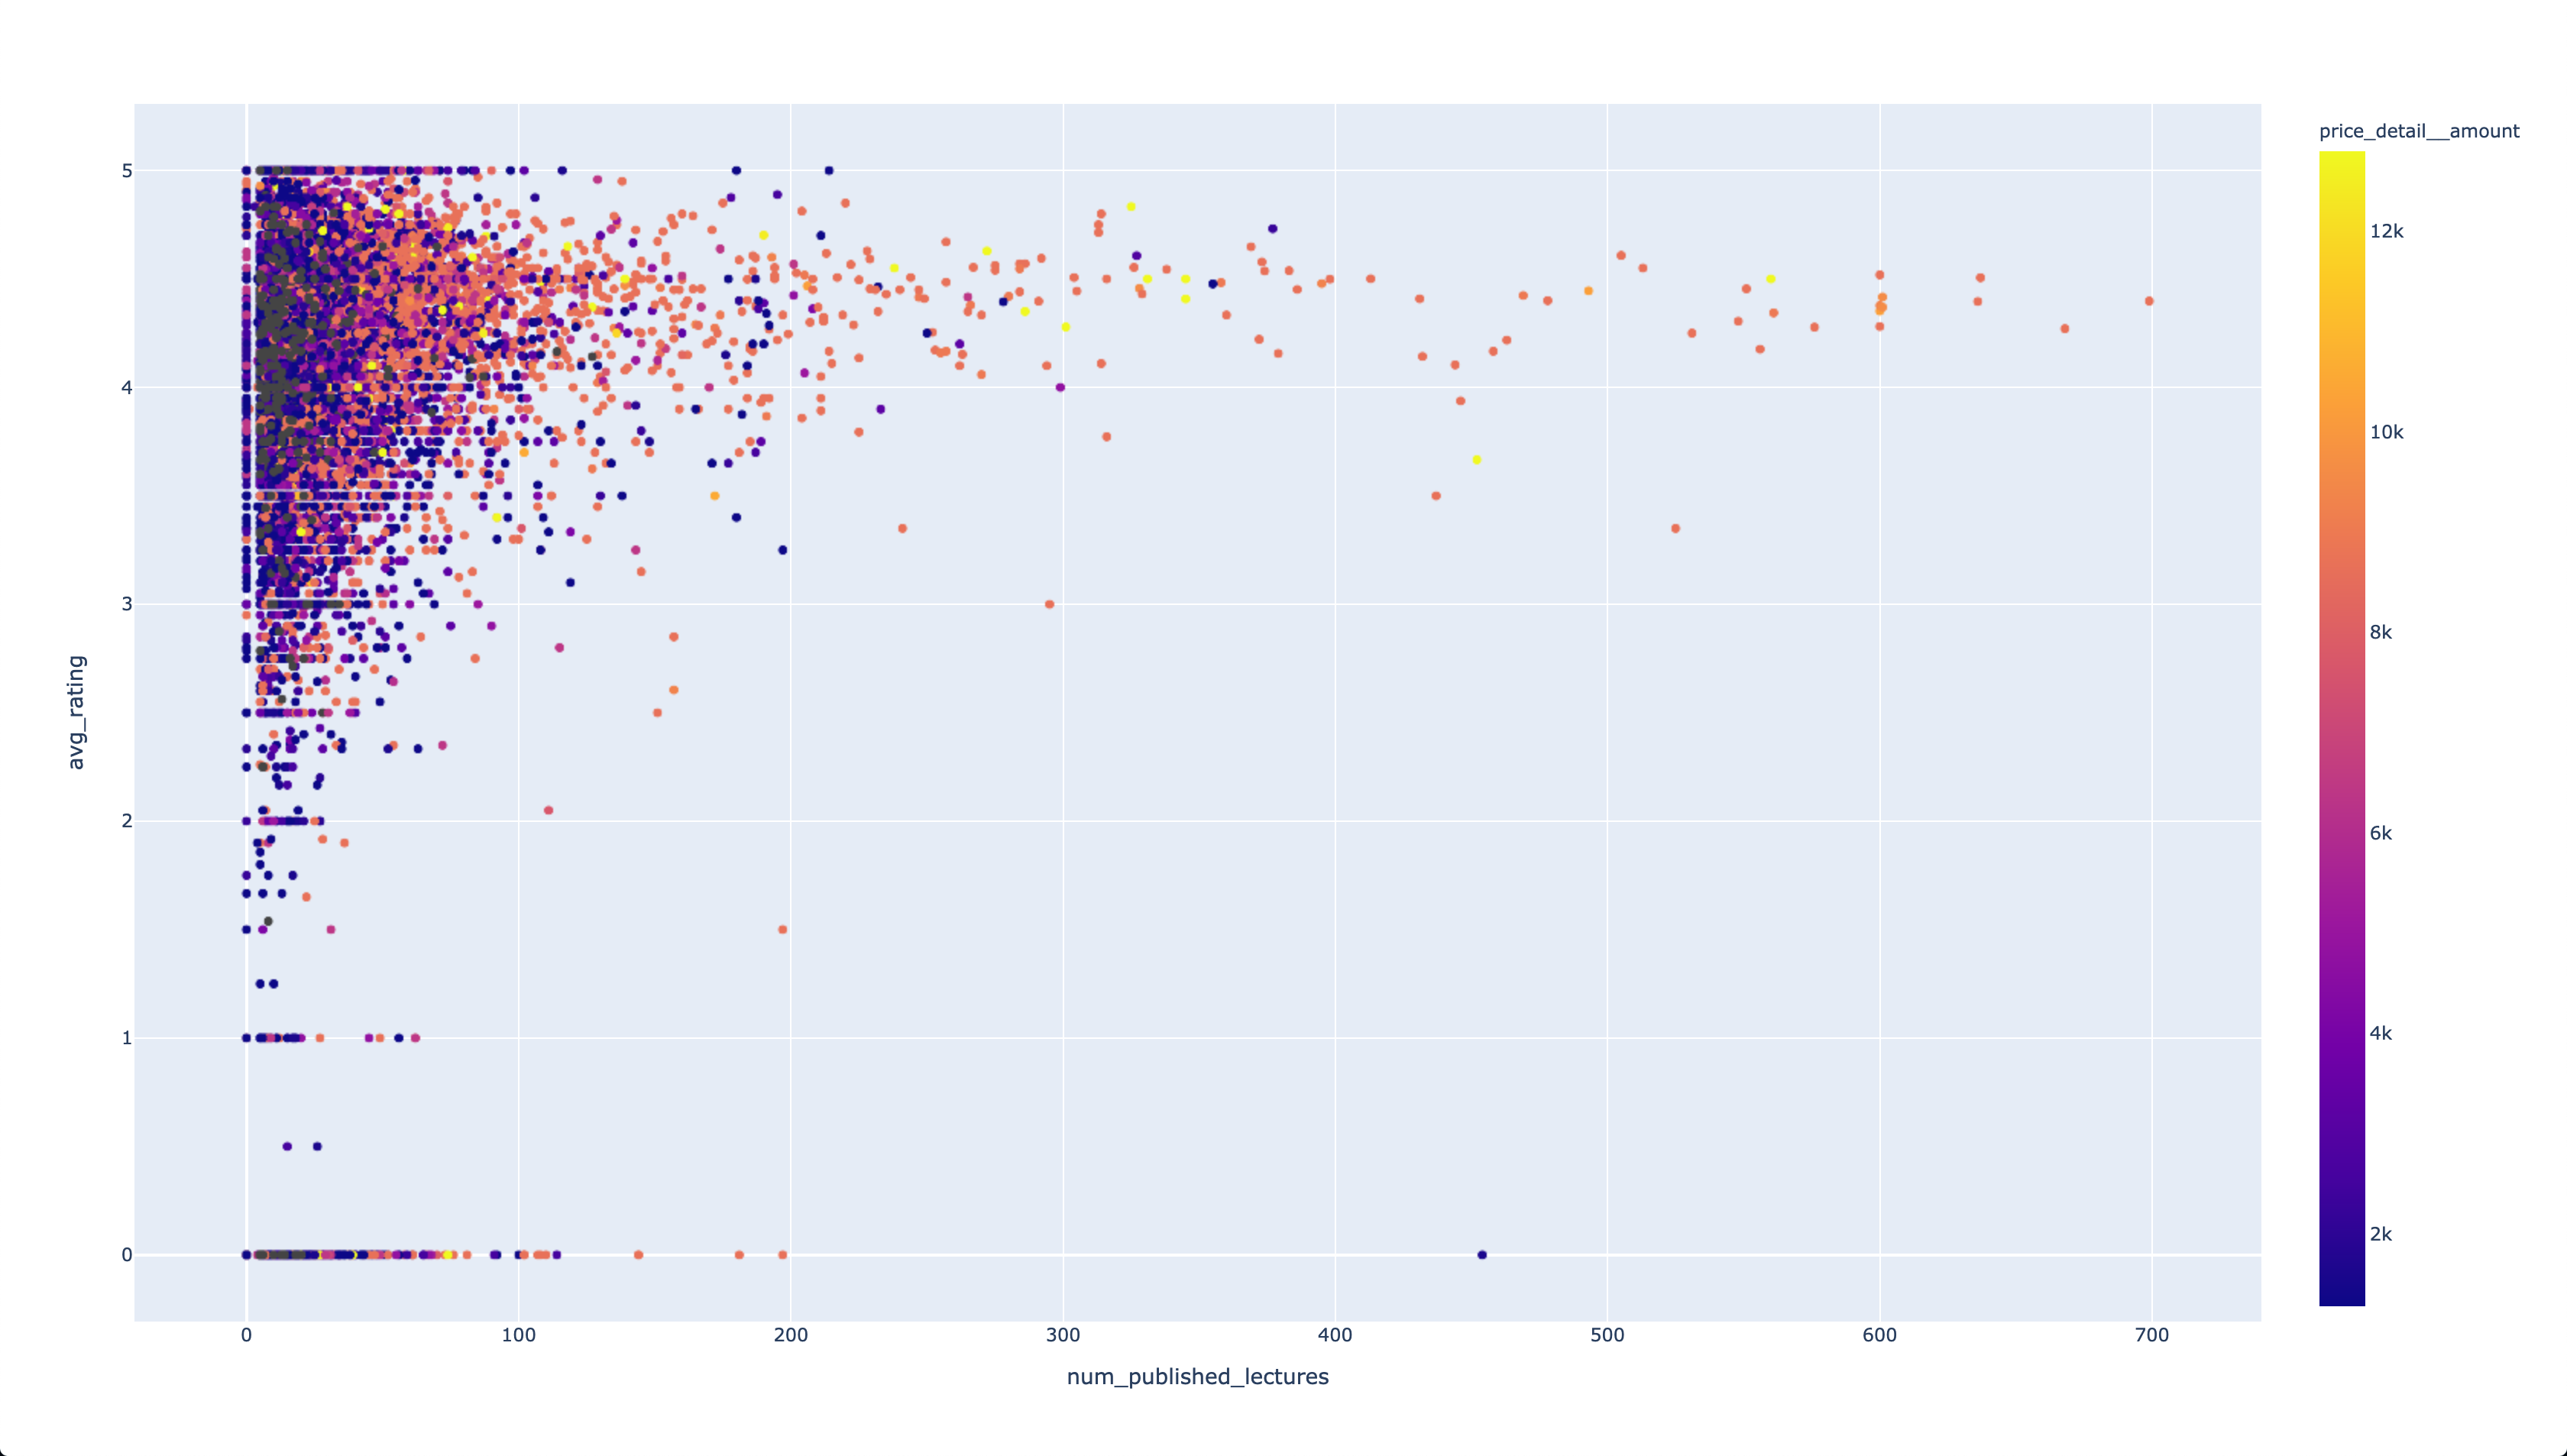
\includegraphics[width=\textwidth]{Screenshot_Index01.png}
\end{figure}

\subsection{Visualization 2}
For this dataset on the best selling books on Amazon from 2009 to 2019, I chose to make a grouped box plot. Since this is a timeseries dataset, I wanted to display that on the x-axis, and see the general trend of reviews. There are also two well defined groups: fiction and non-fiction, and I wanted to see if there were any noticeable disparities between the two. The end result is a grouped box plot. I like this because it shows statistical measures of user rating. For instance, we can see that fiction book are almost always rated more highly than non-fiction.  Along with the boxes, there are also strip plots. These dots show the individual data points of the books. The user can hover a point to see all the information about a book. Like visualization 1, the user can also zoom and re-size as earlier mentioned. Finally, the user can click on a genre listed in the legend to filter it out: clicking on fiction will convert the plot to one of only non-fiction. Clicking on it again will bring it back. 

One of the things I found most interesting about this plot was that many of the best selling books had not been published the same year, but rather may have been from many years ago. For instance, one of the best selling books of 2016 was \href{https://en.wikipedia.org/wiki/To_Kill_a_Mockingbird}{To Kill a Mockingbird}, which was in fact published in 1960. From manual inspection of a few years, I was unable to find this pattern in any non-fiction books. Perhaps there are many classic fiction books which sell well in any year, and relatively few classic non-fiction books that continue to sell well. 

\begin{figure}[htb]
\caption{Visualization for Dataset 2: Amazon Best Selling Books 2009-2019}
\centering
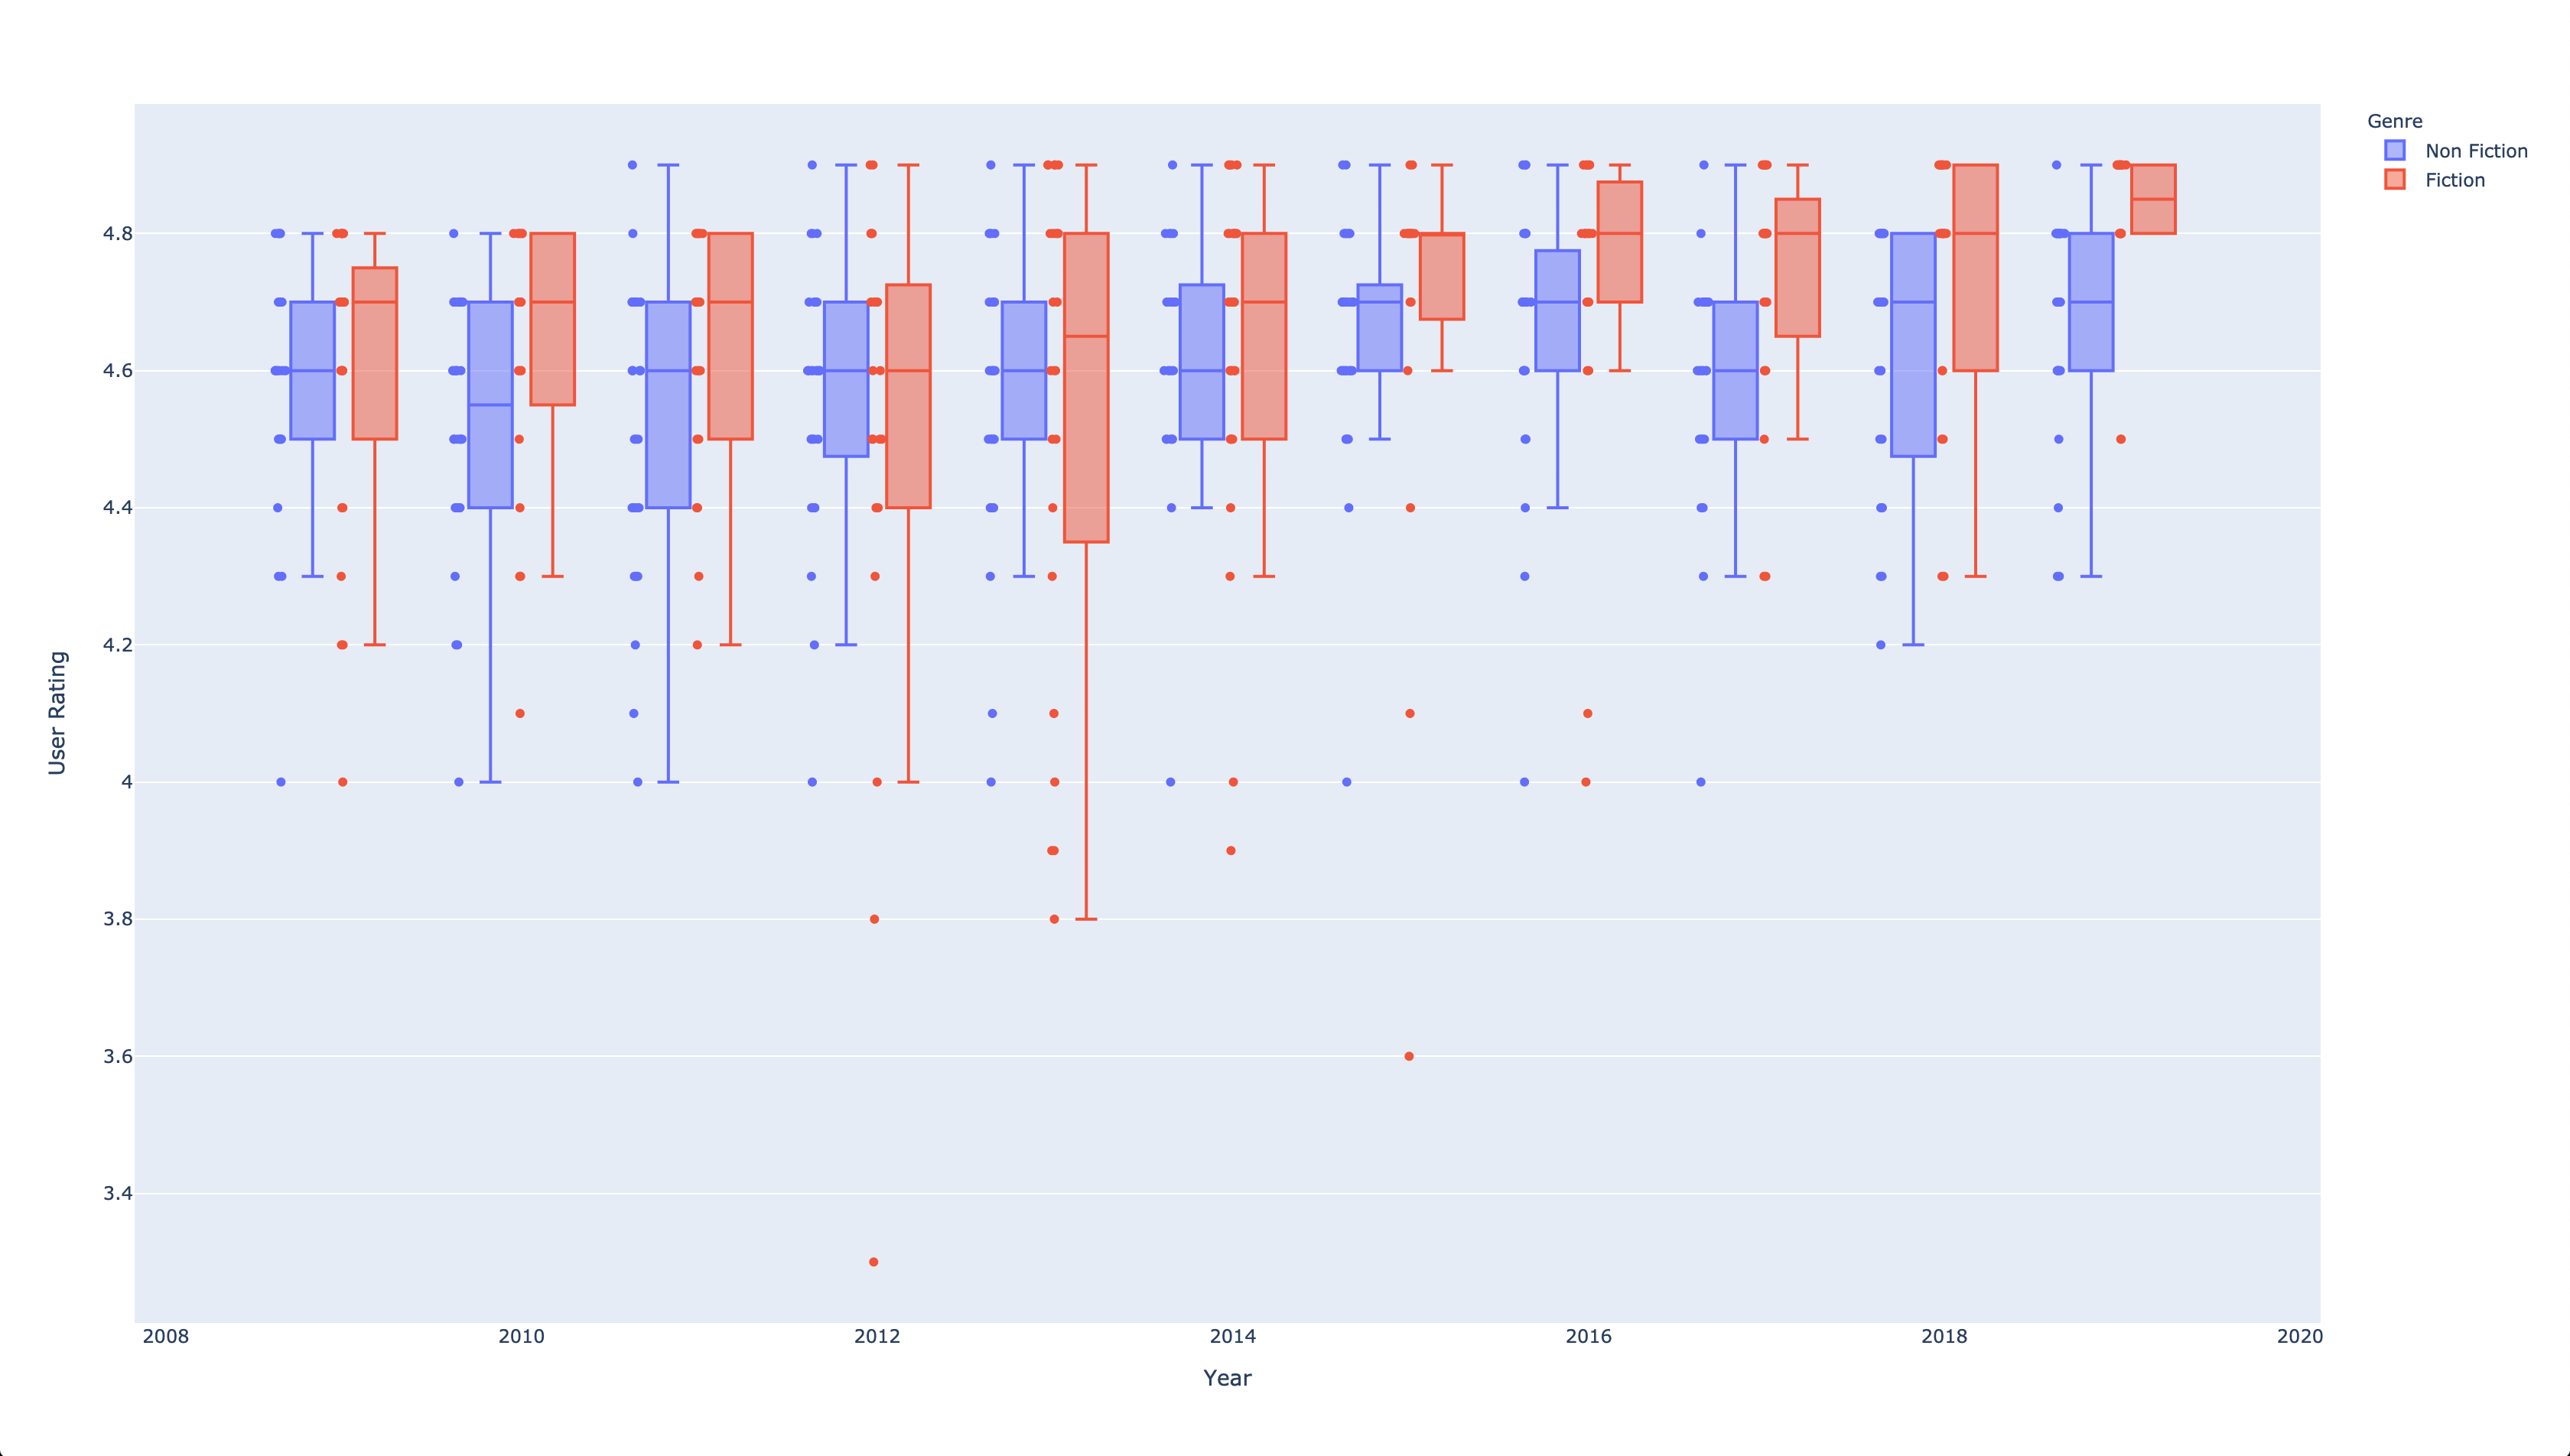
\includegraphics[width=\textwidth]{Screenshot_Index02.png}
\end{figure}

\subsection{Visualization 3}
This dataset contains the geographic data of airports, and their relative traffic levels to pre-COVID times over 215 days. 
Time was again a primary dimension of this dataset, but I wanted the user to interact with the time dimension more viscerally. To do this, I created an animation of the baseline traffic over time. As time progresses and the level of traffic changes, the size of the dot representing each airport changes. 

This visualization leads to a few insights. 
\begin{enumerate}
    \item Most airports' traffic fluctuates a fair amount over time. Could this be due to weekend vs. weekday travel differences?
    \item Hawaii's Daniel K. Inouye International Airport fluctuated much less than most other airports. Is leisure travel relatively steady during COVID? I was under the impression that business travel was less affected than leisure travel. 
    \item On day of year 251 (September 7) almost all airports had drastically reduced traffic compared to the days around them. I was not able to spot this pattern again while watching the data. What happened on September 7?
\end{enumerate}

\begin{figure}[htb]
\caption{Visualization for Dataset 3: COVID19's Impact on Airport Traffic}
\centering
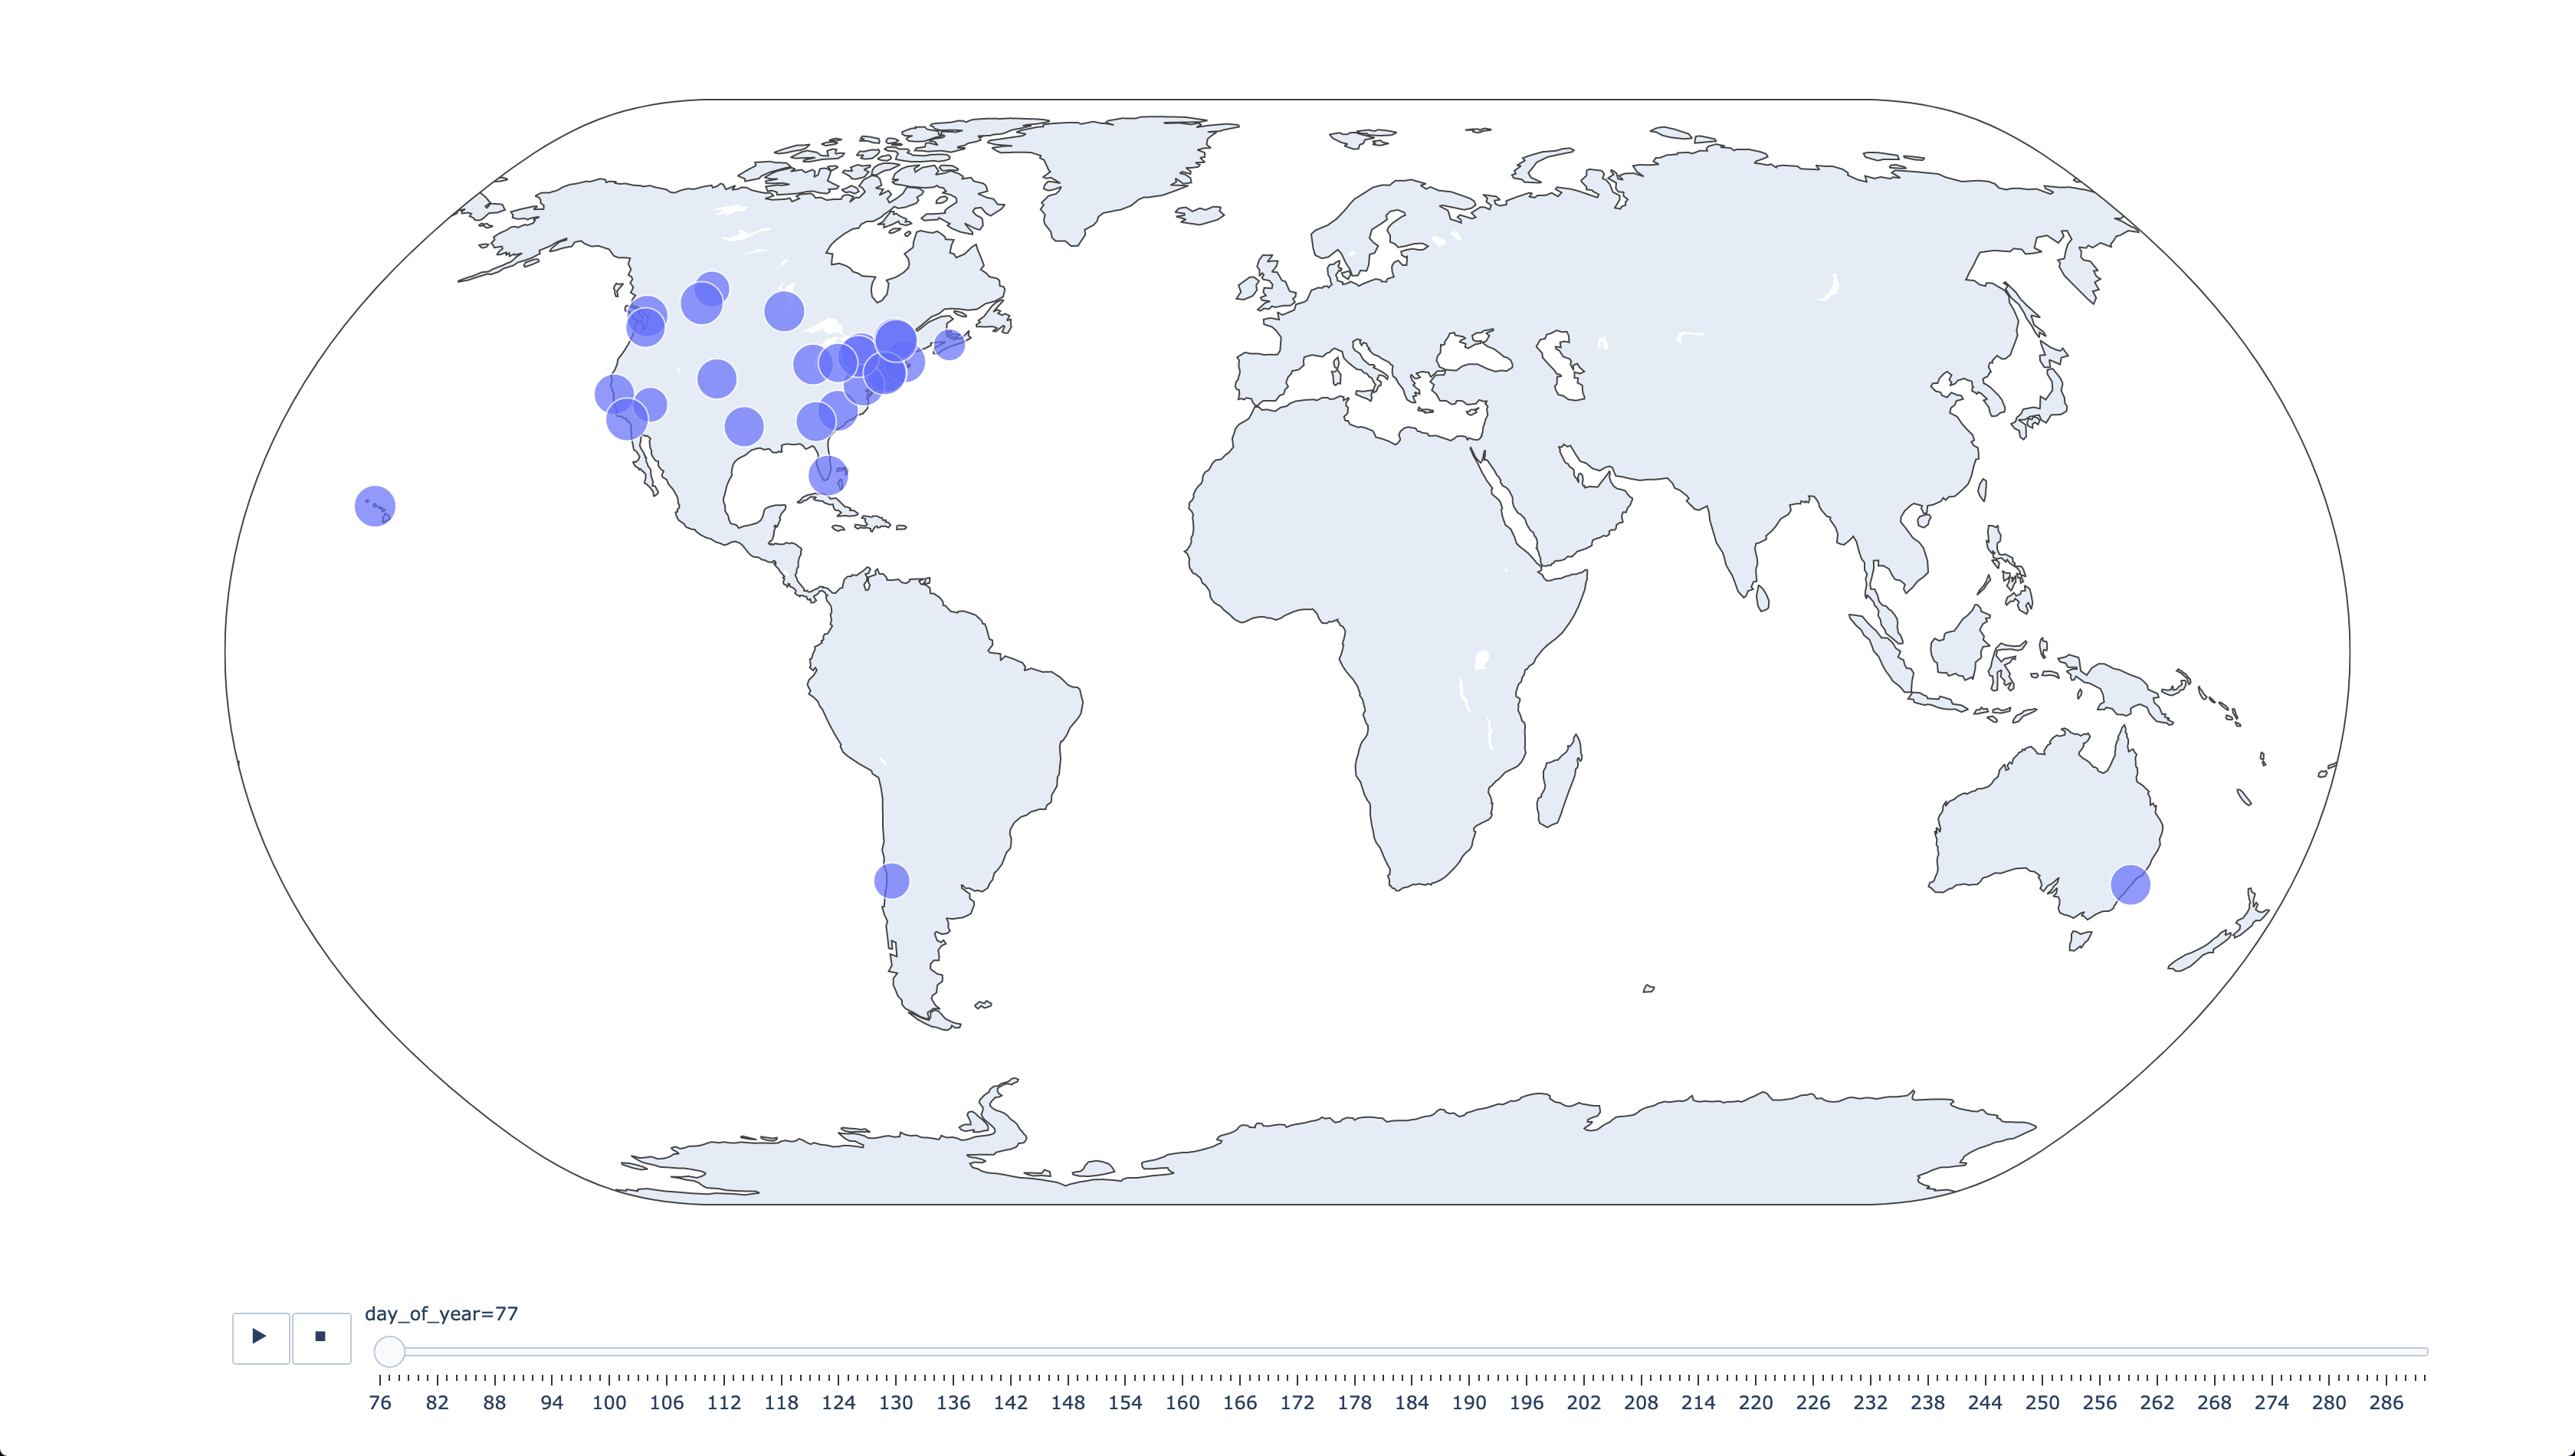
\includegraphics[width=\textwidth]{Screenshot_Index03.png}
\end{figure}

\end{document}
